%NO MODIFICAR ESTA SECCION!
\documentclass{article} % Define la clase del documento, en este caso, un artículo

\usepackage[letterpaper,margin=3cm]{geometry} % Configura el tamaño del papel y los márgenes del documento
\usepackage{graphicx} % Permite la inserción de imágenes
\usepackage[spanish]{babel}% Activar esta configuración para informes en español, ajusta el idioma del documento
\usepackage[usenames]{color} % Permite el uso de colores definidos por nombre en el documento
\usepackage{hyperref} % Habilita enlaces y referencias dentro del documento
\hypersetup{colorlinks=true, linkcolor = black, citecolor= black} % Configura el color de los enlaces y citas
\usepackage{booktabs} % Proporciona comandos para crear tablas de alta calidad
\usepackage{natbib} % Permite el uso de citas y referencias bibliográficas con diferentes estilos
\usepackage{tikz} % Permite la creación de gráficos y diagramas vectoriales directamente en LaTeX
\usepackage{float} % Para controlar la posición de los elementos flotantes, como imágenes, con la opción [H]
\bibliographystyle{agsm} % Define el estilo de citas y bibliografía (en este caso, el estilo AGSM)
\usepackage{diagbox} % Permite crear celdas con líneas diagonales en tablas
\usepackage{listings} % Permite la inclusión y formateo de código fuente en el documento
\usepackage{xcolor} % Paquete para definir y usar colores en el documento
\usepackage{parskip} % Añade espacio entre párrafos en lugar de sangrías
\usepackage{fancyhdr} % Permite personalizar encabezados y pies de página
\usepackage{amsmath} % Proporciona una amplia variedad de entornos y comandos matemáticos
\usepackage{enumitem}
\usepackage{tcolorbox}

% Definimos colores
\definecolor{levelone}{RGB}{230, 230, 250}   % lavanda claro
\definecolor{leveltwo}{RGB}{255, 228, 225}   % rosa claro
\definecolor{levelthree}{RGB}{224, 255, 255} % cian claro
\definecolor{levelfour}{RGB}{240, 255, 240}  % verde claro

\newtcolorbox{highlightbox}[1][]{colback=#1, colframe=white, boxrule=0pt, arc=0pt, left=2pt, right=2pt, top=2pt, bottom=2pt}

\pagestyle{fancy} % Usa el estilo fancyhdr
\fancyhf{} % Borra todos los encabezados y pies de página
\renewcommand{\headrulewidth}{0pt}
\renewcommand{\footrulewidth}{0pt} % Desactiva la línea horizontal predeterminada en el pie
\setlength{\headheight}{2cm} % Ajusta la altura del encabezado para hacer espacio para la línea
\fancyhead[L]{\raisebox{0.20cm}{\textbf{Fluid Mechanics}}} % Añade el texto en la parte izquierda del encabezado, subiéndolo ligeramente
\fancyhead[R]{\raisebox{0.1cm}{
\includegraphics[width=0.25\linewidth]{LOGO_UNIVERSIDAD.jpg}}} % Añade la imagen en la parte derecha del encabezado y súbela un poco
\fancyhead[C]{\rule{\textwidth}{0.6pt}} % Añade una línea horizontal superior centrada
\fancyfoot[C]{\rule{\textwidth}{0.6pt}} % Añade una línea horizontal en el pie de página centrada
\fancyfoot[R]{\raisebox{-1.5\baselineskip}{\thepage}} % Coloca el número de página a la derecha, con suficiente espacio debajo de la línea
\geometry{top=3cm, bottom=2.5cm} % Ajusta los márgenes superior e inferior

% Definición de colores al estilo Visual Studio Code
\definecolor{codegreen}{rgb}{0.25,0.49,0.48} % Comentarios
\definecolor{codegray}{rgb}{0.5,0.5,0.5} % Números y anotaciones
\definecolor{codepurple}{rgb}{0.58,0,0.82} % Palabras clave
\definecolor{backcolour}{rgb}{0.95,0.95,0.92} % Color de fondo

% Configuración del estilo de las celdas de código
\lstset{
    backgroundcolor=\color{backcolour},   % color de fondo; necesita que el paquete color o xcolor esté cargado
    commentstyle=\color{codegreen},       % estilo de comentarios
    keywordstyle=\color{codepurple},      % estilo de palabras clave
    numberstyle=\tiny\color{codegray},    % estilo de los números de línea
    stringstyle=\color{red},              % estilo de las cadenas de texto
    basicstyle=\ttfamily\small,           % estilo del texto básico
    breakatwhitespace=false,              % ajustes de líneas sólo en espacios en blanco
    breaklines=true,                      % ajustar las líneas si son muy largas
    captionpos=b,                         % posición de la leyenda (abajo)
    keepspaces=true,                      % preserva los espacios en el texto; útil si se usa monoespaciado
    numbers=left,                         % dónde poner los números de línea
    numbersep=5pt,                        % qué tan lejos están los números de línea del código
    showspaces=false,                     % mostrar espacios con subrayados particulares; reemplaza 'showstringspaces'
    showstringspaces=false,               % subrayar los espacios dentro de las cadenas solo
    showtabs=false,                       % mostrar tabulaciones en el código con subrayados particulares
    tabsize=2,                            % tamaños de tabulación a 2 espacios
    language=TeX,                         % lenguaje del código
    morecomment=[l]\#,                    % reconocer # como inicio de comentario en Python
    frame=single,                         % agregar un marco simple alrededor del código
    rulecolor=\color{black}               % color del marco
}

\begin{document}
%----------------------------------------------------------------------------------------
%   PORTADA
%Modificar desde aqui en adelante
%----------------------------------------------------------------------------------------
\begin{titlepage}%Inicio de la carátula, solo modificar los datos necesarios
\newcommand{\HRule}{\rule{\linewidth}{0.5mm}} 
\center 
%----------------------------------------------------------------------------------------
%	ENCABEZADO
%----------------------------------------------------------------------------------------

\includegraphics[width=10cm]{LOGO_UNIVERSIDAD.jpg}\\ % Si esta plantilla se copio correctamente, va a llevar la imagen del logo de la facultad.OBS: Es necesario incluir el paquete: graphicx
\vspace{3cm}
%----------------------------------------------------------------------------------------
%	SECCION DEL TITULO
%----------------------------------------------------------------------------------------
\HRule \\[0.4cm]
{ \huge \bfseries Tittle}\\[0.4cm] % Titulo del documento
{ \huge \bfseries Fluid Mechanics}\\[0.4cm] % Titulo del documento
\HRule \\[1.5cm]
 \vspace{5cm}
%----------------------------------------------------------------------------------------
%	SECCION DEL AUTOR
%----------------------------------------------------------------------------------------
\begin{flushright}
    { \textbf{Profesors:}\\
    Patricio Moreno\\
    Sebastian Sepulveda\\
    \vspace{0.2cm}
    \textbf{Assistant:}\\
    Lukas Wolff\\
    \vspace{0.2cm}
    \textbf{Author:}\\
    Pepe\\
}
\end{flushright}
\vspace{1cm}
%----------------------------------------------------------------------------------------
%	SECCION DE LA FECHA
%----------------------------------------------------------------------------------------
{\large \textbf{\today}}\\[2cm] % El comando \today coloca la fecha del dia, y esto se actualiza con cada compilacion, en caso de querer tener una fecha estatica, reemplazar el \today por la fecha deseada
\end{titlepage}
%----------------------------------------------------------------------------------------
%  INDICE
%----------------------------------------------------------------------------------------
\newpage
\tableofcontents
\thispagestyle{plain} % Deshabilita el encabezado en la página del índice
\thispagestyle{empty} % Deshabilita el número de página en la página del índice
\newpage

%Se puede agregar un indice de figuras si es nesesario
%\newpage
%\listoffigures 
%\thispagestyle{plain} % Deshabilita el encabezado en la página del índice %
%\thispagestyle{empty}
%\newpage
%----------------------------------------------------------------------------------------
%   ACÁ EMPIEZA EL INFORME
\setcounter{page}{1} % Reinicia el contador de páginas
%----------------------------------------------------------------------------------------
%Este es el formato a seguir para los titulos de las secciones
\section{Capitulo 1}

\subsection{Proyecto}

\begin{itemize}[label={},left=0pt,align=parleft]
    \item \begin{highlightbox}[levelone] Es un conjunto de actividades relacionadas entre sí \end{highlightbox}
    \item \begin{highlightbox}[levelone] Los proyectos son únicos \end{highlightbox}
    \item \begin{highlightbox}[levelone] Relaciona un equipo de trabajo, en un periodo de tiempo bajo requisitos específicos \end{highlightbox}
\end{itemize}

\subsection{Tipos de Proyectos}

\begin{itemize}[label={},left=0pt,align=parleft]
    \item \begin{highlightbox}[levelone] Proyectos de Construcción \end{highlightbox}
    \begin{itemize}[label={},left=1em,align=parleft]
        \item \begin{highlightbox}[leveltwo] Es un tipo de proyecto que tiene asignados objetivos, especificaciones, plazo y presupuesto \end{highlightbox}
        \item \begin{highlightbox}[leveltwo] Tipos de construcciones: \end{highlightbox}
        \begin{itemize}[label={},left=2em,align=parleft]
            \item \begin{highlightbox}[levelthree] Habitacional \end{highlightbox}
            \item \begin{highlightbox}[levelthree] No habitacional \end{highlightbox}
            \item \begin{highlightbox}[levelthree] Industrial \end{highlightbox}
            \item \begin{highlightbox}[levelthree] Obras Civiles \end{highlightbox}
        \end{itemize}
        \item \begin{highlightbox}[leveltwo] Tipos de Vida: \end{highlightbox}
        \begin{itemize}[label={},left=2em,align=parleft]
            \item \begin{highlightbox}[levelthree] Vida de Diseño: Es la vista prevista del proyecto, es la que se espera que tenga. \end{highlightbox}
            \item \begin{highlightbox}[levelthree] Vida Útil: Es la duración estimada que un objeto debe tener, respecto a factores externos. \end{highlightbox}
            \item \begin{highlightbox}[levelthree] Vida Remanente: Es el periodo durante el cual un objeto puede utilizarse de forma rentable antes de que la mantención ya no sea viable. \end{highlightbox}
        \end{itemize}
        \item \begin{highlightbox}[leveltwo] Etapas de un Proyecto de Construcción: \end{highlightbox}
        \begin{itemize}[label={},left=2em,align=parleft]
            \item \begin{highlightbox}[levelthree] Existe una necesidad \end{highlightbox}
            \item \begin{highlightbox}[levelthree] Análisis \end{highlightbox}
            \item \begin{highlightbox}[levelthree] Identificación de soluciones \end{highlightbox}
            \item \begin{highlightbox}[levelthree] Estudios de Factibilidad \end{highlightbox}
            \item \begin{highlightbox}[levelthree] Evaluación \end{highlightbox}
            \item \begin{highlightbox}[levelthree] Financiamiento \end{highlightbox}
            \item \begin{highlightbox}[levelthree] Diseño, que considera los siguientes aspectos: \end{highlightbox}
            \begin{itemize}[label={},left=3em,align=parleft]
                \item \begin{highlightbox}[levelfour] Estudio de Terreno \end{highlightbox}
                \item \begin{highlightbox}[levelfour] Diseño Arquitectónico \end{highlightbox}
                \item \begin{highlightbox}[levelfour] Diseño Estructural \end{highlightbox}
                \item \begin{highlightbox}[levelfour] Estudios de Impacto Ambiental \end{highlightbox}
                \item \begin{highlightbox}[levelfour] Diseño de Instalaciones \end{highlightbox}
                \item \begin{highlightbox}[levelfour] Redacción de documentos de licitación \end{highlightbox}
                \item \begin{highlightbox}[levelfour] Constructibilidad y Mantención \end{highlightbox}
            \end{itemize}
            \item \begin{highlightbox}[levelthree] Licitacion \end{highlightbox}
            \item \begin{highlightbox}[levelthree] Construcción \end{highlightbox}
            \item \begin{highlightbox}[levelthree] Puesta en Marcha \end{highlightbox}
        \end{itemize}
    \end{itemize}
\end{itemize}

De esta manera, un proyecto de construcción se puede expresar de la siguiente manera:

\begin{figure}[H]
    \centering
    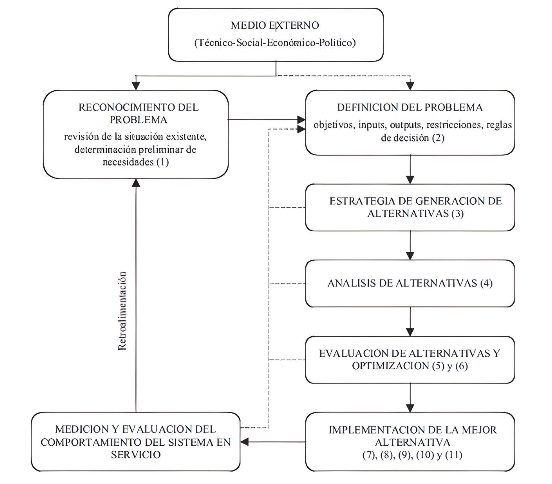
\includegraphics[width=0.5\textwidth]{proyecto_construccion.png}
    \caption{Proyecto de Construcción}
    \label{fig:ProyectoConstruccion}
\end{figure}

\section{Capítulo 2}

\subsection{Diseño de un Proyecto de Construcción}

\begin{itemize}[label={},left=0pt,align=parleft]
    \item \begin{highlightbox}[levelone] Estudio de terreno, el cual consta de: \end{highlightbox}
    \begin{itemize}[label={},left=1em,align=parleft]
        \item \begin{highlightbox}[leveltwo] Ubicación del terreno \end{highlightbox}
        \item \begin{highlightbox}[leveltwo] Condiciones propias tales como: \end{highlightbox}
        \begin{itemize}[label={},left=2em,align=parleft]
            \item \begin{highlightbox}[levelthree] Topografía \end{highlightbox}
            \item \begin{highlightbox}[levelthree] Geología \end{highlightbox}
            \item \begin{highlightbox}[levelthree] Hidrología \end{highlightbox}
            \item \begin{highlightbox}[levelthree] Fuentes de Abastecimiento como energía y comunicaciones \end{highlightbox}
        \end{itemize}
        \item \begin{highlightbox}[leveltwo] Aspectos Legales, específicos a cada zona. \end{highlightbox}
        \item \begin{highlightbox}[leveltwo] Condiciones de servicio, como agua potable, electricidad o alcantarillado. \end{highlightbox}
        \item \begin{highlightbox}[leveltwo] Evaluación de impacto ambiental. \end{highlightbox}
    \end{itemize}
\end{itemize}

\subsection{Leyes}

\begin{itemize}[label={},left=0pt,align=parleft]
    \item \begin{highlightbox}[levelone] Ley general de urbanismo y construcciones (DFL 458, MINVU): Contiene el proceso global de urbanismo y construcción. \end{highlightbox}
    \item \begin{highlightbox}[levelone] Ley Base del Medio Ambiente (Ley 19.300): Regula el derecho a vivir en un medio ambiente libre de contaminación. \end{highlightbox}
    \item Ley para la contruccion de viviendas economicas (DFL-2 de 1959): Desarrollo el concepto de vivienda economica como aquella que tiene max 140 $m^2$ y no excede los 17.5 $m^2$ edificados por cama.
    \item Decreto Ley 2552-1979: Busca resolver los problemas de marginidad habitacional, tambien define el conecpto de vivienda de emergencia.
    \item  Codigo del Trabajo (2002): regula remuneraciones, grafiticaciones, contratos, descanzos, etc.
    \item Ley sobre accidente de trabajo y enfermedades profesionales (16.744): Establece un seguro obligatorio contra accidentes del trabajo y enfermedades profesionales.
    \item Ley de subcontratacion (20.123): Regula la subcontratacion de trabajadores.
    \item Ley de Concesiones (DFL 164) y Reglamento(DS 240) de Conseciones de Obras Publicas: Regula la concesion de obras publicas.
    \item Codigo Civil: El constructor tiene una responsabilidad de 5 años sobre la obra.
    \item Ley de la venta por piso o ley de propiedad horizontal (Ley 6071): Regula la venta de departamentos en construccion.
    \item Ley que incorpora el IVA a las empresas constructoras (Ley 18.630)
    \item etc
\end{itemize}

\subsection{Normas}

INN =$>$ Instituto Nacional de Normalización, cumplir sus normas no es de caracter obligatorio. Algunas de las areas que cubre:

\begin{itemize}
    \item general
    \item Diseño Arquitectonico
    \item Diseño, Calculo y Ejecucion de Estrucutras
    \item acondicionamiento Ambiental
    \item Materiales y Componentes
    \item Instalacones
    \item Herramientas
\end{itemize}

\subsection{Especificaciones Tecnicas}

Corresponden a documentos asociados al proyecto, y sirven como complemento hacia los planos.

\subsection{Permisos y derechos de Construccion}

Las obras privadas deben tener un permisode construccion, antes de comenzar su ejecucion.

\subsection{Permisos de Construccion}

Se solicita a la direccion de obras municipales, para su obtencion, se debe seguir el siguiente proceso:

\begin{itemize}
    \item Solicitud de permiso: firmada por el propietario y arquitecto del proyecto
    \item Legado de documentos, que incluye:
    \begin{itemize}
        \item Fotocopia de certificado y informaciones previas.
        \item Formulario unico de estadisticas de edificacion
        \item Certificado de factibilida de estadisticas
        \item Planos de Arquitectura
        \item Proyecto de calculo estructural
        \item Cuadros de superficie
        \item Especificaciones tecnicas de las pertidas
        \item Levantamiento topografico
    \end{itemize}
    \item Pago de derechos municipales
    \item Firma de documentos
\end{itemize}

\subsection{Sitema de Evaluacion de Impacto Ambiental}





\newpage 

\section{Capítulo 3}
\subsection{Elementos de la gestion de la construccion}

\begin{minipage}{0.45\textwidth}
    \begin{itemize}
        \item Hay que encontrar un balance entre estos 3 items
        \item Una buena gestión de Calidad reducirá los plazos
        \item Una buena gestión de calidad mantendrá o reducirá los costos
    \end{itemize}
\end{minipage}
\hfill
\begin{minipage}{0.45\textwidth}
    \centering
    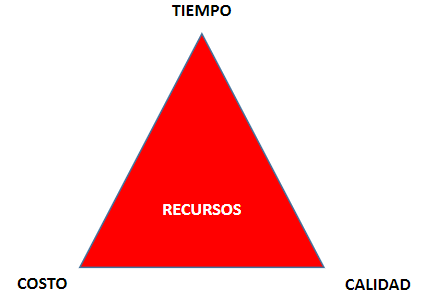
\includegraphics[width=\textwidth]{gestion_recursos.png}
\end{minipage}

\subsection{Factibilidad de un Proyecto de Construcción}
\begin{minipage}{0.45\textwidth}
    \begin{itemize}
        \item No es factible si al planificarlo existe la posibilidad que se sobrepasen límites de plazos o presupuestos
        \item No es factible si no se cuenta con equipos o mano de obra o materiales que garanticen la calidad del proyecto
    \end{itemize}
\end{minipage}
\hfill
\begin{minipage}{0.5\textwidth}
    \centering
    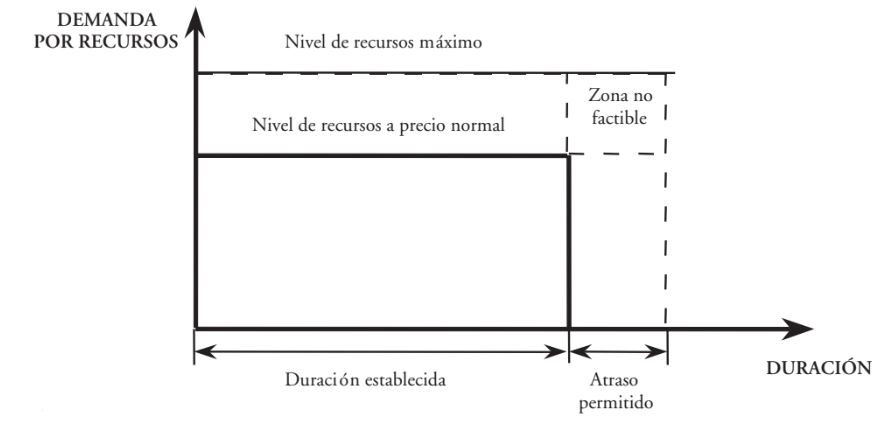
\includegraphics[width=1.2\textwidth]{factibilidad_proyecto.png}
\end{minipage}

\begin{minipage}{0.45\textwidth}
    \begin{itemize}
        \item El proyecto se materializará a través de varias etapas:
        \begin{itemize}
            \item estudio y desarrollo del proyecto de ingeniería definitivo
            \item construcción y puesta en marcha de la obra
        \end{itemize}
    \item La incertidumbre del costo depende de que tan bien se desarrollen las etapas
    \end{itemize}
\end{minipage}
\hfill
\begin{minipage}{0.5\textwidth}
    \centering
    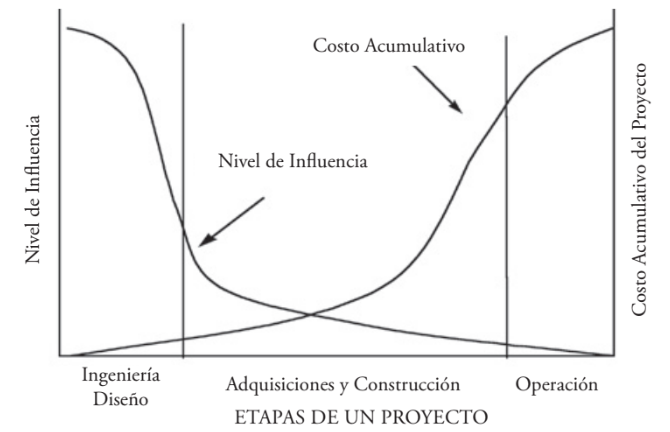
\includegraphics[width=1.2\textwidth]{etapas_proyecto.png}
\end{minipage}

\subsection{Administración de Proyectos}

\begin{minipage}{0.45\textwidth}
    \begin{itemize}
        \item La administración tiene por objetivo transformar una decisión de inversión en una obra física
        \item Especificaciones de los objetivos del proyecto
        \item Maximización de los recursosCoordinación
        \item Coordinación
        \item Comunicación efectiva
    \end{itemize}
\end{minipage}
\hfill
\begin{minipage}{0.5\textwidth}
    \centering
    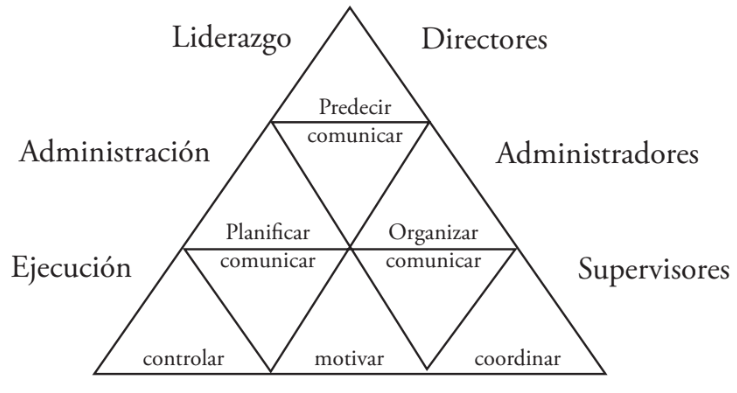
\includegraphics[width=1.2\textwidth]{piramide_administracion.png}
\end{minipage}

\subsection{Mandante y demás participantes}
Ventajas de realizar obras por medio de empresas contratistas:
\begin{itemize}
    \item Se ocupan recursos externos, que son regulados con un contratos
    \item La empresa tiene personal especializado y experiencia en la construcción
    \item La empresa se organiza distribuyendo en las variadas faenas su personal (No los despiden lo trasladan)
    \item Las empresas son más eficientes en:
    \begin{itemize}
        \item Recursos físicos
        \item inversión 
        \item Adquisición de materiales
    \end{itemize}
\end{itemize}

\subsection{Estructuras organizacionales}

\begin{figure}[h!]
    \centering
    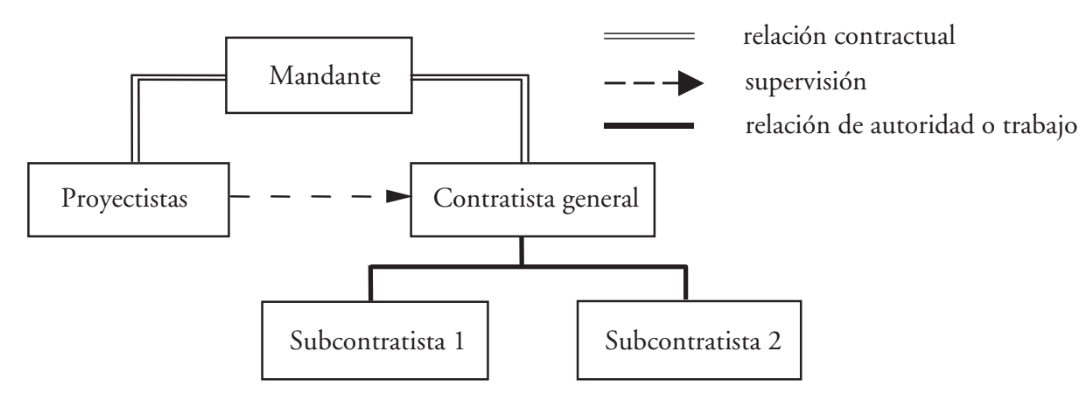
\includegraphics[width=0.9\textwidth]{trad_rel.png}
    \caption{Estructura tradicional}
    \label{fig:estructuras_organizacionale}
\end{figure}

\begin{figure}[h!]
    \centering
    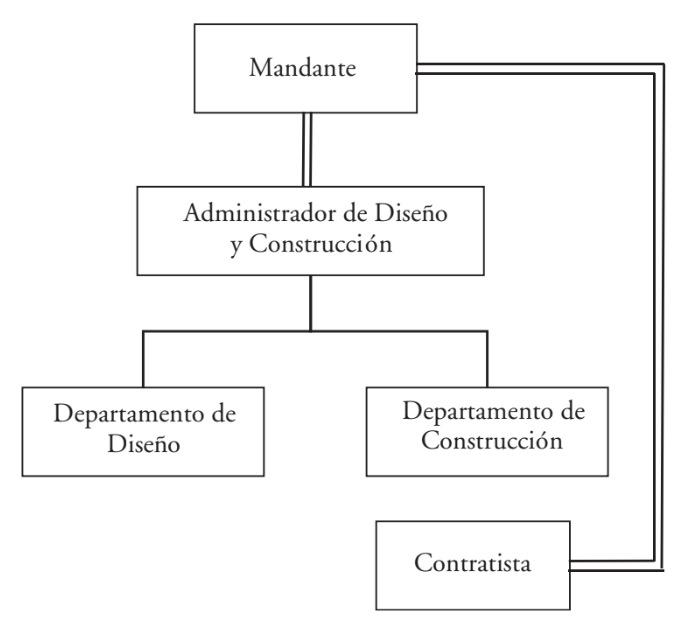
\includegraphics[width=0.5\textwidth]{ad_dis_rel.png}
    \caption{Estructura de administación de diseño y de construcción}
    \label{fig:estructuras_organizacional}
\end{figure}

\begin{figure}[h!]
    \centering
    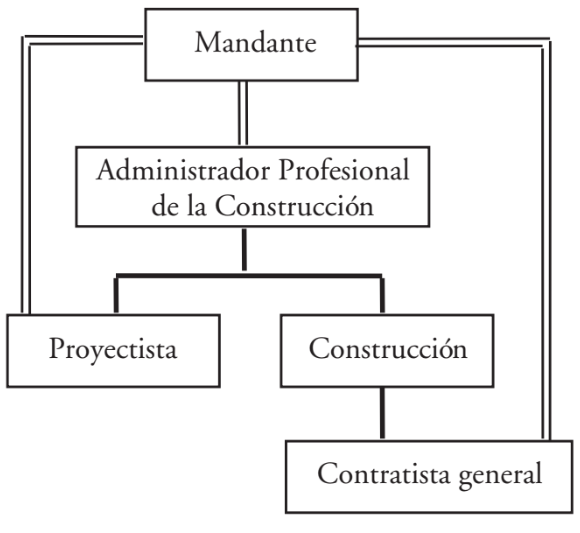
\includegraphics[width=0.5\textwidth]{sd_prof_rel.png}
    \caption{Estructura de administración profesional de la construcción}
    \label{fig:estructuras_organizacionales}
\end{figure}

\begin{figure}[h!]
    \centering
    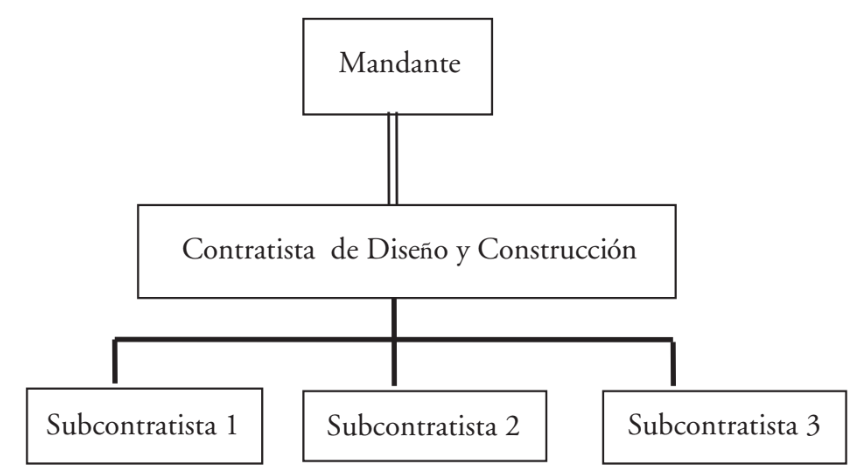
\includegraphics[width=0.45\textwidth]{dis_cons_rel.png}
    \caption{Estructura de administración de diseño y construcción (Llave en mano)} 
    \label{fig:estructura_organizacionales}
\end{figure}

\newpage

\subsection{Estructura de equipo para la ejecución de proyectos}
\begin{minipage}{0.45\textwidth}
    \begin{itemize}
        \item \textbf{Organización por coordinación}
        \item El proyecto es llevado por las respectivas áreas funcionales, asesoradas por un coordinador
    \end{itemize}
\end{minipage}
\hfill
\begin{minipage}{0.5\textwidth}
    \centering
    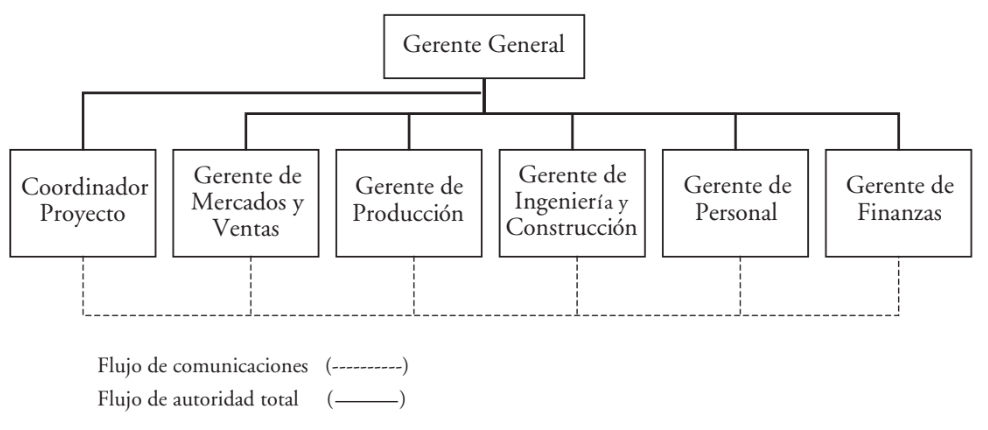
\includegraphics[width=1.2\textwidth]{Arbol_org_proyecto.png}
\end{minipage}

\begin{minipage}{0.45\textwidth}
    \begin{itemize}
        \item \textbf{Organización pura del proyecto}
        \item Se crea una organización funcional especial para el proyecto
        \item Esta organización es paralela a la existente en la empresa
        \item Aumento de costos debido a la organización paralela
        \item Se aplica en proyectos realizados en zonas geográficas alejadas de centros gerenciales
    \end{itemize}
\end{minipage}
\hfill
\begin{minipage}{0.5\textwidth}
    \centering
    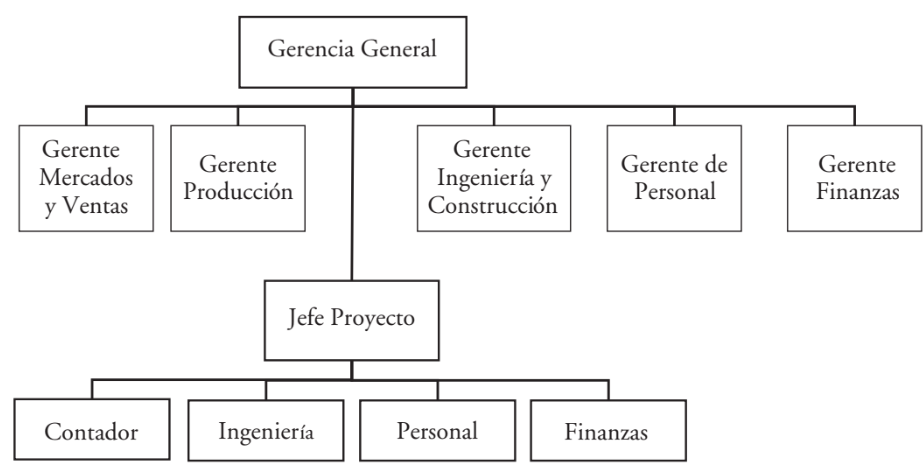
\includegraphics[width=1.2\textwidth]{arbol_org_gen.png}
\end{minipage}

\begin{minipage}{0.45\textwidth}
    \begin{itemize}
        \item \textbf{Organización matricial}
        \item Maximizar el uso de recusos disponibles
        \item Toma de decisiones más lenta
        \item Útil en proyectos con fuertes restricciones de presupuesto
    \end{itemize}
\end{minipage}
\hfill
\begin{minipage}{0.5\textwidth}
    \centering
    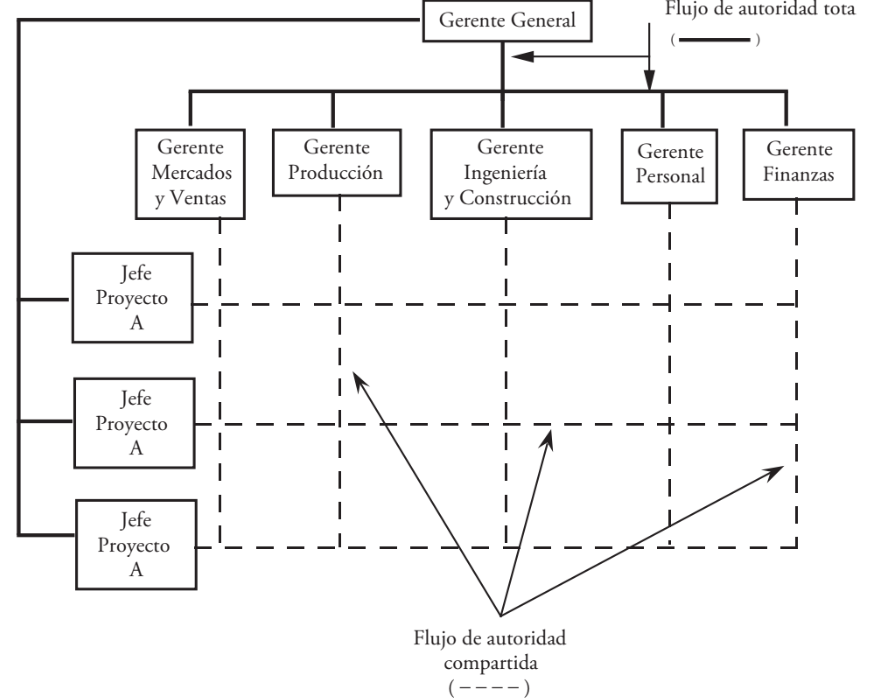
\includegraphics[width=1\textwidth]{matriz_proyecto.png}
\end{minipage}

\begin{minipage}{0.45\textwidth}
    \begin{itemize}
        \item \textbf{Organización semipura del proyecto}
        \item Sistema intermedio entre el matricial y el puro

    \end{itemize}
\end{minipage}
\hfill
\begin{minipage}{0.5\textwidth}
    \centering
    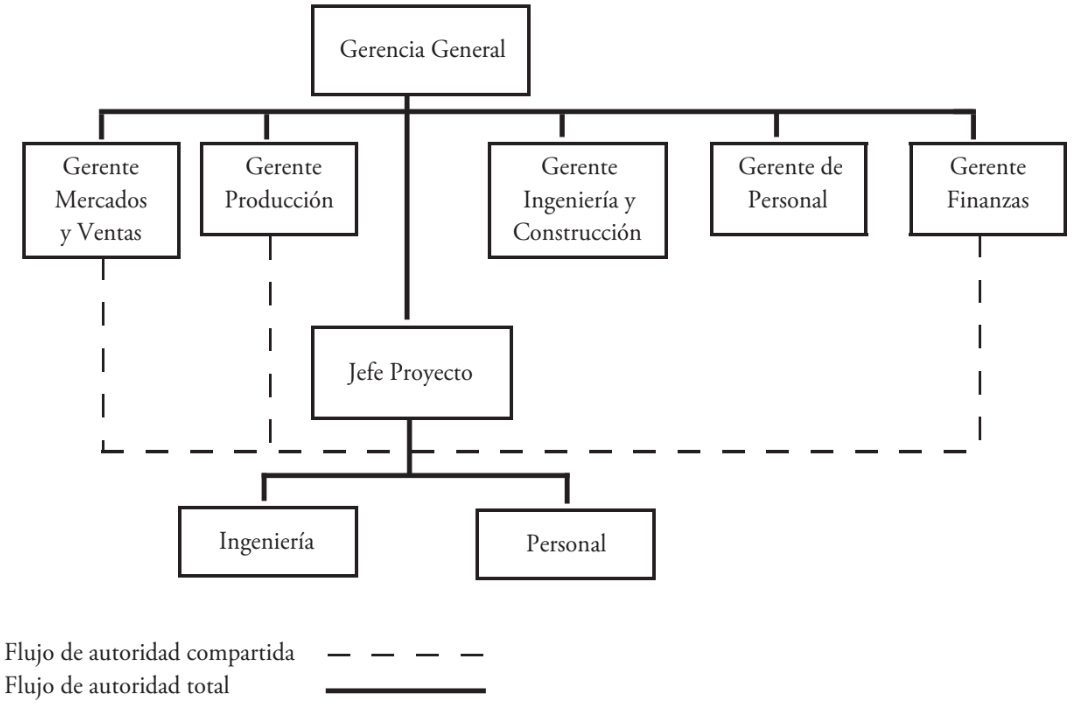
\includegraphics[width=1\textwidth]{org_semipura_proyecto.png}
\end{minipage}

\newpage

\subsection{Planificación y control de proyectos de obras de construcción}  
\begin{itemize}
    \item Racionalizar las actividades del proceso constructivo
    \item Racionalizar los recursos y establecesr control de estos
    \item Benficios:
    \begin{itemize}
        \item Reducir incertidumbre
        \item Conocer los volumenes peak
        \item Programar los movimientos de la instalación y retiro de faena 
        \item Optimizar la programación de área de la obra
        \item Elaborar un programa de adquisiciones de materiales y arriendo de equipos
        \item Definir periodos de contratos y despidos
        \item Establecer metodologías de control
    \end{itemize}
\end{itemize}

\subsubsection{Niveles de planificación}
\begin{itemize}
    \item \textbf{Planificación estratégica}
    \begin{itemize}
        \item Se realiza a largo plazo
        \item Se establecen los aspectos globales del proyecto
        \item Se determinan costos estimados para propuestas
    \end{itemize}
    \item \textbf{Planificación táctica}
    \begin{itemize}
        \item Se realiza a mediano plazo
        \item Planifica la materialización del proyecto
        \item Plan de construcción de general a detalle
    \end{itemize}
    \item \textbf{Planificación operativa}
    \begin{itemize}
        \item Se realiza a corto plazo
        \item Como ejecutar las tareas necesarias para materializar las etapas del proyecto
        \item Nivel de detalle: planificación semanañ o inclusive diaria
    \end{itemize}
\end{itemize}


\subsection{Metodología de planificación}
Consiste en realizar un desglose de actividades para luego establecer secuencialidad, desfases y simultaneidad. (Carta Gant)

\subsection{Gestión y control de costos de proyectos}
Incluye los procesos necesarios para asegurar que el proyecto se finalice dentro del presupuesto aprobado.
\begin{itemize}
    \item Planificación de recursos
    \item Estimación de costos
    \item Presupuesto de costos
    \item Control de costos
    \item Costos del ciclo de vida del proyecto
    \begin{itemize}
        \item Limitación de revisiones del diseño disminuye costos del proyecto, pero aumenta los costos de operación y mantención del mandante
    \end{itemize}
    \item Tasa iterna de retorno (TIR)
    \item Valor actualizado neto (VAN)
    \item Periodo de recuperación del capital
\end{itemize}

\subsection{Planificación de los recursos}
\begin{itemize}
    \item Determinación de recursos
    \item Estructura de descomposición del proyecto
    \item Utilización de resultados previos
    \item Uso de información histórica
    \item Disponibilidad de recursos
    \item Herramientas de planificación
    \item Juicio experto
    \item Resultado de la planificación de recursos
\end{itemize}
\subsubsection{Estimación de costos}
\begin{itemize}
    \item Aproximación de costos
    \item Diferencia entre estimación de costos y fijación de precio
    \item Identificación de costos alternativos
    \item Uso de la estructura de descomposición del proyecto
    \item Conocimiento de precios unitarios de los recursos
    \item Estimación de la duración de las actividades
    \item Uso de información histórica
    \item Herramientas para la estimación de costos
    \begin{itemize}
        \item Estimación por analogías
        \item Modelización paramétrica
        \item Estimación de abajo hacia arriba
        \item Herramientas computarizadas
    \end{itemize}
    \item Actividades de apoyo para la estimación de costos
    \item Plan de gestión de costos
\end{itemize}

\subsection{Presupuesto de costos}
\begin{itemize}
    \item Asignación de estimaciones de costos a tareas individuales
    \item Base de costos para medir el comportamiento del proyecto
    \item Estructura de descomposición del proyecto y programa del proyecto
    \item Presupuesto por fases temporales
    \item Curva de la "S" para medir y controlar los costos del proyecto
\end{itemize}

\subsection{Control de costos}


\begin{minipage}{0.45\textwidth}
    \begin{itemize}
    \item Influencia en factores que causan cambios en la base de costos
    \item Control del desarrollo de los costos
    \item Garantía de reflejar cambios apropiados en la base de costos
    \item Prevención de cambios incorrectos o inapropiados
    \item Comunicación de cambios autorizados a entidades involucradas
    \end{itemize}
\end{minipage}
\hfill
\begin{minipage}{0.5\textwidth}
    \centering
    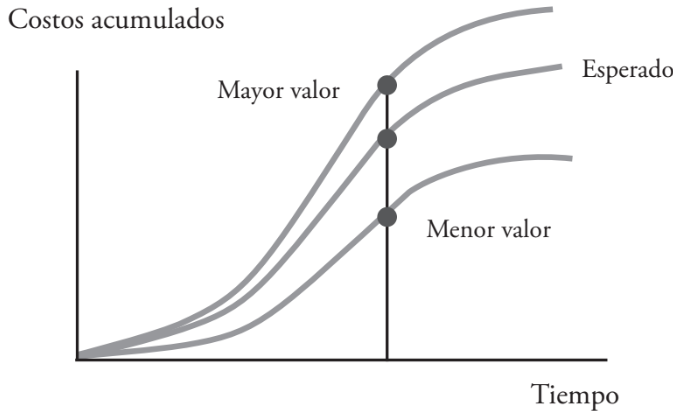
\includegraphics[width=\textwidth]{curva_s.png}
\end{minipage}
























\end{document}




